\begin{document}
\title{\Large \lecture \\ \textbf{\normalsize \assignment}}
\author{\authors}

\setlength \headheight{25pt}
\fancyhead[R]{\begin{tabular}{r}\lecture \\ \assignment \end{tabular}}
\fancyhead[L]{\authors}




\maketitle

\section{Introduction}
The goal of this project is to transfer textfiles as sequence of characters through a network with reliable data transfer. In this paper we will present our layering and protocol design of milestone~\ifthenelse{\boolean{m2}}{2}{3}.

\section{Layering and Protocol Design}

Beside the two layers, physical and application layer, cnet provides we implement three additional layers between them. We call them \emph{link layer}, \emph{network layer}, and \emph{transport layer}, from bottom to top. Data packets in the link layer are called \emph{frame}, in the network layer \emph{datagram} and in the transport layer \emph{segment}. To data packets from the application layer we refer to as \emph{messages}.


\subsection{Link Layer}
\begin{figure}
  \centering
  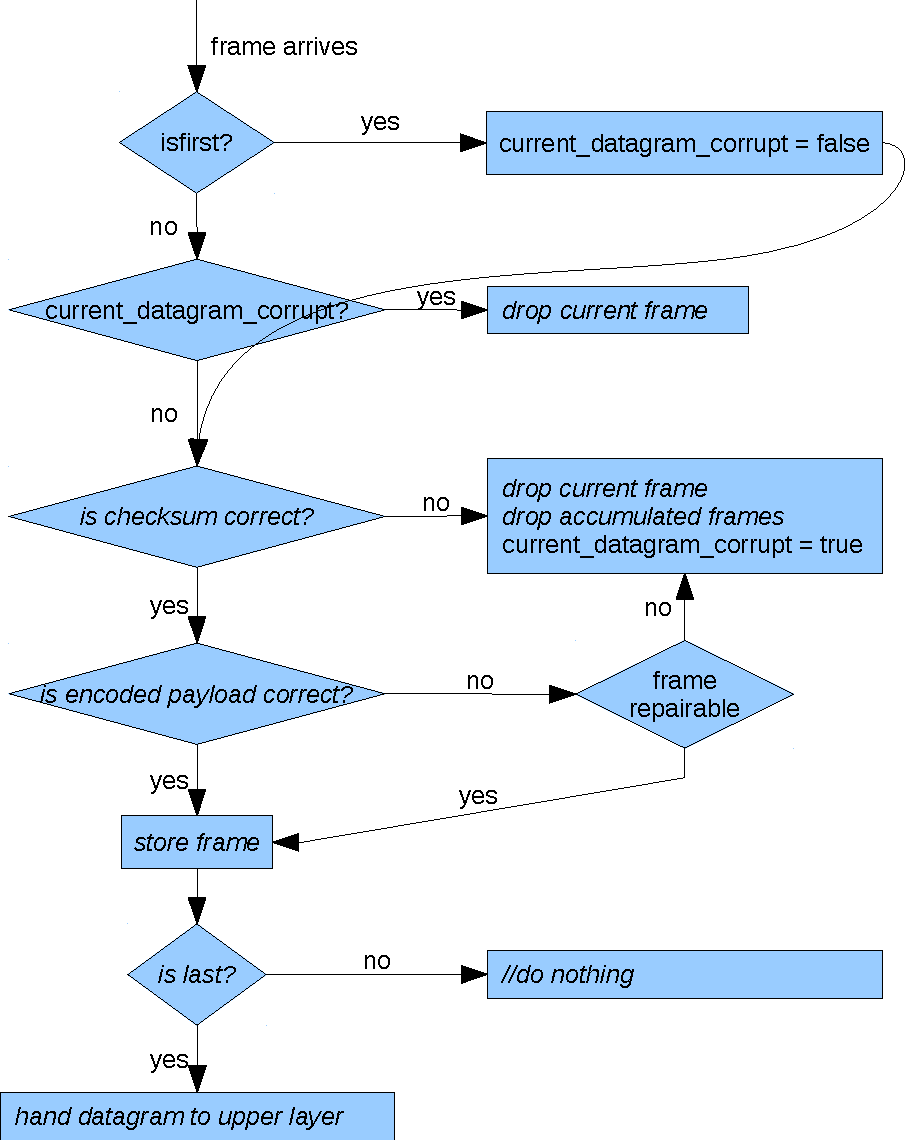
\includegraphics[width=0.9\textwidth]{images/flowgraph_link_layer_receiver.pdf}
  \caption[Receiver side of link layer]{\hcaption{Receiver side of link layer.} The flow graph shows how data on the receiver side of the link layer are handled.}
  \label{fig:receiver-side-link-layer}
\end{figure}
The link layer provides basic "point2point" connections between neighboring nodes. It can handle the transmission of arbitrary large packets (limited by the buffer size, which is large enough to handle all messages in this scenario) independently of the MTU of the link because it has the ability of fra(g)mentation. This means that data from the upper layer are split into several frames which fit to the MTU and put together on the receiver side. This mechanism is guarded by the fact that no reordering of frames on one link occur. This layer also guarantees that all datagram which are handed to the upper layer are \emph{free of corruption}. Corrupt frames are recognized by computing a checksum and all frames with errors which are not repairable are dropped. \fixme{will we implement error handling} Finally, the data in this layer are handed to the physical layer in a first come first serve fairness. Figure~\ref{fig:receiver-side-link-layer} illustrates the receiver side of the link layer.


\subsection{Network Layer}
\ifthenelse{\boolean{m2}}{ %text for milestone 2
  In the second milestone the network layer has no function. It only hands the data from the upper layer to the lower one and vice versa. It will get the function of maintaining and building a routing / forwarding table as well as route datagrams through the network.

}{%test for milestone 3
  The network layer has two main tasks: build and maintain a routing / forwarding table as well as route datagrams through the network. The building and maintaining of the routing table is done in a distributed fashion. Initially only the costs to the direct neighbors is known and all other costs are infinite. The minimal costs are broadcasted to the direct neighbors. If a node receives information of a lower cost path, it updates it forwarding table. If the minimal route cost changes it broadcasts this again to its neighbors.

  The forwarding table is build from the routing table by choosing the neighbor with the minimal costs. If a datagram arrives at a node, the network layer decides if it is the final destination of the datagram or if the datagram needs to be forwarded on the basis of the forwarding table. On each hop a datagram takes, the hop counter is decreased to avoid that a datagram travels too long in the network.
}




\subsection{Transport Layer}
\ifthenelse{\boolean{m2}}{% text for milestone 2
  In the second milestone the transport layer has no function. It only hands the data from the upper layer to the lower one and vice versa. It will get the function to guarantee reliable data transfer, congestion and flow control, segment messages to decrease the number of resend messages in case of corruption. To improve throughput it will buffer reordered messages.
}{% text for milestone 3
  The main task of the transport layer is to provide reliable data transfer. This means that only corruption free messages are delivered in order to the application layer. To provide this service, the transport layer uses cumulative acknowledgments and sequence numbers in form of offsets. For each received or send message from a host a connection is created. This contains a buffer for incoming data, cyclic sequence numbers and information to detect if messages are received complete. A window is used to send multiple messages without waiting for each acknowledgment. To increase performance we use cumulative acknowledgments where the acknowledgment number is the next offset the connection is waiting for. To provide this in an efficient way we buffer a limited amount of reordered messages.
  
  Additionally this layer provides congestion and flow control \fixme{how?}.
  
  Due to smaller MTU than the size of the messages we additionally segment messages on this layer to decrease the number of resend messages in case of corruption. If a frame on the link layer gets corrupt, we need to resend the whole segment the whole path the frames are reached previously without errors. If the segments are smaller, the traffic becomes lower.

}

\end{document}